\documentclass[11pt]{article}
\usepackage[margin=1in]{geometry}
\usepackage{amsmath,amssymb}
\usepackage{array,booktabs}
\usepackage{tikz}
\usepackage{enumitem}

\setlength{\parindent}{0pt}
\setlength{\parskip}{6pt}

\begin{document}

\begin{center}
    {\Large \textbf{Practice Final Exam Solutions (STAT 461)}}
\end{center}

\section*{Problem 1}

\textbf{Question.} The world population has recently crossed the 7.5 billion mark, but approximately 1 in 8 people in the world today remain undernourished or malnourished. If 120 people are randomly selected, find the chances that there are (a) at least 5, (b) at most 9, and (c) between 10 and 20 inclusive undernourished or malnourished people in the sample.

\textbf{Solution.} Let
\[
X=\text{number of undernourished or malnourished people in the sample}.
\]
Since approximately 1 in 8 people are undernourished or malnourished,
\[
p=\frac{1}{8}=0.125, \qquad n=120.
\]
Thus
\[
X\sim \operatorname{Binomial}(120,0.125).
\]
Since
\[
np=120(0.125)=15, \qquad n(1-p)=120(0.875)=105,
\]
the binomial distribution may be approximated by a normal distribution:
\[
X\approx N\left(np, np(1-p)\right)=N(15,13.125).
\]
Therefore,
\[
\mu=15, \qquad \sigma=\sqrt{13.125}\approx 3.6228.
\]

\textbf{(a)} Using a continuity correction,
\[
P(X\ge 5)=P(X>4.5).
\]
Thus,
\[
P(X\ge 5)\approx P\left(Z>\frac{4.5-15}{3.6228}\right)=P(Z>-2.899).
\]
Therefore,
\[
\boxed{P(X\ge 5)\approx 0.9981}.
\]

\textbf{(b)} Using a continuity correction,
\[
P(X\le 9)=P(X<9.5).
\]
Thus,
\[
P(X\le 9)\approx P\left(Z<\frac{9.5-15}{3.6228}\right)=P(Z<-1.518).
\]
Therefore,
\[
\boxed{P(X\le 9)\approx 0.0645}.
\]

\textbf{(c)} Using a continuity correction,
\[
P(10\le X\le 20)=P(9.5<X<20.5).
\]
Thus,
\[
P(10\le X\le 20)\approx P\left(\frac{9.5-15}{3.6228}<Z<\frac{20.5-15}{3.6228}\right).
\]
That is,
\[
P(10\le X\le 20)\approx P(-1.518<Z<1.518).
\]
Therefore,
\[
\boxed{P(10\le X\le 20)\approx 0.8710}.
\]

\newpage
\section*{Problem 2}

\textbf{Question.} If $X$, $Y$, and $Z$ are independent random variables with means $15$, $22$, and $10$ respectively and standard deviations $2$, $5$, and $7$ respectively, find the mean and the standard deviation of $3X+2Y-4Z$.

\textbf{Solution.} Let
\[
W=3X+2Y-4Z.
\]
Using linearity of expectation,
\[
E(W)=3E(X)+2E(Y)-4E(Z).
\]
Substituting the given means,
\[
E(W)=3(15)+2(22)-4(10)=45+44-40=49.
\]
Thus,
\[
\boxed{\mu_W=49}.
\]

Since $X,Y,Z$ are independent,
\[
\operatorname{Var}(W)=3^2\operatorname{Var}(X)+2^2\operatorname{Var}(Y)+(-4)^2\operatorname{Var}(Z).
\]
Using the given standard deviations,
\[
\operatorname{Var}(X)=2^2=4, \qquad \operatorname{Var}(Y)=5^2=25, \qquad \operatorname{Var}(Z)=7^2=49.
\]
Therefore,
\[
\operatorname{Var}(W)=9(4)+4(25)+16(49)=36+100+784=920.
\]
So,
\[
\boxed{\sigma_W=\sqrt{920}=2\sqrt{230}\approx 30.33}.
\]

\newpage
\section*{Problem 3}

\textbf{Question.} If $X_1,\ldots,X_n$ are i.i.d. Standard Beta$(3,5)$ random variables, find the mean and variance of
\[
X=\sum_{i=1}^n(c_iX_i+b_i),
\]
for constants $c_1,\ldots,c_n$ and $b_1,\ldots,b_n$.

\textbf{Solution.} For a Beta$(\alpha,\beta)$ random variable,
\[
E(X_i)=\frac{\alpha}{\alpha+\beta},
\qquad
\operatorname{Var}(X_i)=\frac{\alpha\beta}{(\alpha+\beta)^2(\alpha+\beta+1)}.
\]
Here, $\alpha=3$ and $\beta=5$. Thus,
\[
E(X_i)=\frac{3}{3+5}=\frac{3}{8},
\]
and
\[
\operatorname{Var}(X_i)=\frac{(3)(5)}{(3+5)^2(3+5+1)}=\frac{15}{64(9)}=\frac{15}{576}=\frac{5}{192}.
\]

Now,
\[
E(X)=E\left[\sum_{i=1}^{n}(c_iX_i+b_i)\right].
\]
By linearity of expectation,
\[
E(X)=\sum_{i=1}^{n}\left(c_iE(X_i)+b_i\right).
\]
Therefore,
\[
\boxed{E(X)=\sum_{i=1}^{n}\left(\frac{3c_i}{8}+b_i\right)}.
\]

Since $X_1,\ldots,X_n$ are independent,
\[
\operatorname{Var}(X)=\operatorname{Var}\left[\sum_{i=1}^{n}(c_iX_i+b_i)\right]=\sum_{i=1}^{n}c_i^2\operatorname{Var}(X_i).
\]
Thus,
\[
\boxed{\operatorname{Var}(X)=\frac{5}{192}\sum_{i=1}^{n}c_i^2}.
\]

\newpage
\section*{Problem 4}

\textbf{Question.} Durations of 911 phone calls are skewed to the right, with population mean $12$ minutes and population standard deviation $3.2$ minutes. For a simple random sample of $64$ calls, find the approximate distribution of the sample average. Then find the chances that the sample average (a) exceeds $13$ minutes and (b) is below $10.8$ minutes.

\textbf{Solution.} Let $X$ denote the duration of a randomly selected 911 phone call. The given values are
\[
\mu=12, \qquad \sigma=3.2, \qquad n=64.
\]
Although the population distribution is skewed to the right, the sample size is large enough to use the Central Limit Theorem. Thus,
\[
\bar X\approx N\left(\mu,\frac{\sigma^2}{n}\right).
\]
Therefore,
\[
\bar X\approx N\left(12,\frac{3.2^2}{64}\right)=N(12,0.16).
\]
Equivalently,
\[
\boxed{\bar X\approx N(12,0.4^2)}.
\]

\textbf{(a)}
\[
P(\bar X>13)=P\left(Z>\frac{13-12}{0.4}\right)=P(Z>2.5).
\]
Thus,
\[
P(\bar X>13)=1-\Phi(2.5)\approx 1-0.9938=0.0062.
\]
Therefore,
\[
\boxed{P(\bar X>13)\approx 0.0062}.
\]

\textbf{(b)}
\[
P(\bar X<10.8)=P\left(Z<\frac{10.8-12}{0.4}\right)=P(Z<-3).
\]
Thus,
\[
P(\bar X<10.8)=\Phi(-3)\approx 0.0013.
\]
Therefore,
\[
\boxed{P(\bar X<10.8)\approx 0.0013}.
\]

\newpage
\section*{Problem 5}

\textbf{Question.} Let $Y_1,\ldots,Y_{36}$ be a simple random sample from a Poisson$(\mu=9)$ population. What is the approximate distribution of $2(\bar Y-9)$? So, what is $P(|\bar Y-9|\le 1.5)$?

\textbf{Solution.} For a Poisson random variable,
\[
E(Y_i)=\mu=9, \qquad \operatorname{Var}(Y_i)=\mu=9.
\]
The sample mean is
\[
\bar Y=\frac{1}{36}\sum_{i=1}^{36}Y_i.
\]
By the Central Limit Theorem,
\[
\bar Y\approx N\left(\mu,\frac{\sigma^2}{n}\right)=N\left(9,\frac{9}{36}\right)=N\left(9,\frac14\right).
\]
Thus,
\[
\bar Y-9\approx N\left(0,\frac14\right).
\]
Therefore,
\[
2(\bar Y-9)\approx N(0,1).
\]
So,
\[
\boxed{2(\bar Y-9)\approx N(0,1)}.
\]

Now,
\[
P(|\bar Y-9|\le 1.5)=P(-1.5\le \bar Y-9\le 1.5).
\]
Multiplying all parts by $2$,
\[
P(|\bar Y-9|\le 1.5)=P(-3\le 2(\bar Y-9)\le 3).
\]
Since $2(\bar Y-9)\approx Z$,
\[
P(|\bar Y-9|\le 1.5)\approx P(-3\le Z\le 3).
\]
Using the standard normal table,
\[
P(-3\le Z\le 3)=\Phi(3)-\Phi(-3)\approx 0.9987-0.0013=0.9974.
\]
Hence,
\[
\boxed{P(|\bar Y-9|\le 1.5)\approx 0.9974}.
\]

\newpage
\section*{Problem 6}

\textbf{Question.} In a poll of $n=1100$ adults, $517$ said they favored legalizing marijuana. Write down a $90\%$ confidence interval and a $99\%$ confidence interval for the true population proportion supporting legalization.

\textbf{Solution.} Let $p$ be the true unknown population proportion of adults who support legalizing marijuana. The given values are
\[
n=1100, \qquad x=517.
\]
Thus,
\[
\hat p=\frac{x}{n}=\frac{517}{1100}=0.47.
\]
Also,
\[
1-\hat p=0.53.
\]

For a large-sample confidence interval for a population proportion,
\[
\hat p\pm z_{\alpha/2}\sqrt{\frac{\hat p(1-\hat p)}{n}}.
\]
First compute the standard error:
\[
SE=\sqrt{\frac{\hat p(1-\hat p)}{n}}=\sqrt{\frac{(0.47)(0.53)}{1100}}\approx 0.01505.
\]

\textbf{90\% Confidence Interval.} For a $90\%$ confidence interval,
\[
z_{\alpha/2}=z_{0.05}=1.645.
\]
Therefore,
\[
0.47\pm 1.645(0.01505)=0.47\pm 0.02475.
\]
Thus,
\[
\boxed{(0.4453,0.4947)}.
\]

\textbf{99\% Confidence Interval.} For a $99\%$ confidence interval,
\[
z_{\alpha/2}=z_{0.005}=2.576.
\]
Therefore,
\[
0.47\pm 2.576(0.01505)=0.47\pm 0.03877.
\]
Thus,
\[
\boxed{(0.4312,0.5088)}.
\]

\newpage
\section*{Problem 7}

\textbf{Question.} How large a sample size is needed to estimate an unknown population proportion of ``yes'' answers by a $99\%$ confidence interval whose width is $0.4$?

\textbf{Solution.} For a confidence interval for a population proportion,
\[
\hat p\pm z_{\alpha/2}\sqrt{\frac{\hat p(1-\hat p)}{n}}.
\]
The width of the interval is $2E$, where $E$ is the margin of error. The desired width is $0.4$, so
\[
2E=0.4 \qquad \Longrightarrow \qquad E=0.2.
\]
Since the population proportion is unknown, use the conservative value
\[
\hat p=0.5.
\]
Thus,
\[
\hat p(1-\hat p)=(0.5)(0.5)=0.25.
\]
For a $99\%$ confidence interval,
\[
z_{\alpha/2}=z_{0.005}=2.576.
\]
The required sample size satisfies
\[
E=z_{\alpha/2}\sqrt{\frac{\hat p(1-\hat p)}{n}}.
\]
Solving for $n$,
\[
n=\frac{z_{\alpha/2}^2\hat p(1-\hat p)}{E^2}.
\]
Substituting,
\[
n=\frac{(2.576)^2(0.25)}{(0.2)^2}=\frac{6.6358(0.25)}{0.04}=41.474.
\]
Since the sample size must be rounded up,
\[
\boxed{n=42}.
\]

\newpage
\section*{Problem 8}

\textbf{Question.} If a random sample of size $15$ is taken from a Normal population with mean $75$, what are the chances that
\[
\left(\frac{\bar X-75}{S/\sqrt{15}}\right)
\]
exceeds $2.145$ in absolute value?

\textbf{Solution.} Since the population standard deviation is not given, use the sample standard deviation $S$. Then
\[
T=\frac{\bar X-\mu}{S/\sqrt{n}}
\]
has a Student's $t$-distribution with
\[
n-1=15-1=14
\]
degrees of freedom. Here,
\[
T=\frac{\bar X-75}{S/\sqrt{15}}\sim t_{14}.
\]
Find
\[
P\left(\left|\frac{\bar X-75}{S/\sqrt{15}}\right|>2.145\right)=P(|T|>2.145).
\]
From the $t$-table with $14$ degrees of freedom,
\[
t_{0.025,14}=2.145.
\]
Therefore,
\[
P(T>2.145)=0.025.
\]
By symmetry of the $t$-distribution,
\[
P(|T|>2.145)=2P(T>2.145)=2(0.025)=0.05.
\]
Hence,
\[
\boxed{P\left(\left|\frac{\bar X-75}{S/\sqrt{15}}\right|>2.145\right)=0.05}.
\]

\newpage
\section*{Problem 9}

\textbf{Question.} Suppose $Y_1,\ldots,Y_n$ are a simple random sample from a Uniform$[0,\theta]$ population. What is the method-of-moments estimate of $\theta$? What is the method-of-moments estimate of $\theta^2$?

\textbf{Solution.} For a Uniform$[0,\theta]$ random variable,
\[
E(Y_i)=\frac{0+\theta}{2}=\frac{\theta}{2}.
\]
The first moment equation is
\[
\bar Y=\frac{\theta}{2}.
\]
Solving for $\theta$,
\[
\boxed{\hat\theta_{\text{MOM}}=2\bar Y}.
\]

For a Uniform$[0,\theta]$ random variable,
\[
\operatorname{Var}(Y_i)=\frac{(\theta-0)^2}{12}=\frac{\theta^2}{12}.
\]
Equating this to the sample variance,
\[
S^2=\frac{1}{n-1}\sum_{i=1}^{n}(Y_i-\bar Y)^2,
\]
gives
\[
S^2=\frac{\theta^2}{12}.
\]
Solving for $\theta^2$,
\[
\boxed{\widehat{\theta^2}_{\text{MOM}}=12S^2}.
\]

\newpage
\section*{Problem 10}

\textbf{Question.} If $X_1,X_2,\ldots,X_n$ are a simple random sample from a Weibull$(3,\beta)$ population, derive the maximum likelihood estimate of $\beta$.

\textbf{Solution.} The Weibull density is
\[
f(x)=\frac{\alpha}{\beta^\alpha}x^{\alpha-1}e^{-(x/\beta)^\alpha}, \qquad x>0.
\]
Since $\alpha=3$,
\[
f(x)=\frac{3}{\beta^3}x^2e^{-(x/\beta)^3}, \qquad x>0.
\]

The likelihood function is
\[
L(\beta)=\prod_{i=1}^{n}\frac{3}{\beta^3}x_i^2e^{-(x_i/\beta)^3}.
\]
Thus,
\[
L(\beta)=\frac{3^n}{\beta^{3n}}\left(\prod_{i=1}^{n}x_i^2\right)\exp\left(-\sum_{i=1}^{n}\frac{x_i^3}{\beta^3}\right).
\]
The log-likelihood function is
\[
\ell(\beta)=\ln L(\beta)=n\ln 3-3n\ln\beta+2\sum_{i=1}^{n}\ln x_i-\frac{\sum_{i=1}^{n}x_i^3}{\beta^3}.
\]
Differentiate with respect to $\beta$:
\[
\frac{d\ell}{d\beta}=-\frac{3n}{\beta}+\frac{3\sum_{i=1}^{n}x_i^3}{\beta^4}.
\]
Set this equal to $0$:
\[
-\frac{3n}{\beta}+\frac{3\sum_{i=1}^{n}x_i^3}{\beta^4}=0.
\]
Multiplying by $\beta^4$,
\[
-3n\beta^3+3\sum_{i=1}^{n}x_i^3=0.
\]
Therefore,
\[
n\beta^3=\sum_{i=1}^{n}x_i^3,
\]
so
\[
\beta^3=\frac{1}{n}\sum_{i=1}^{n}x_i^3.
\]
Hence,
\[
\hat\beta_{\text{MLE}}=\sqrt[3]{\frac{1}{n}\sum_{i=1}^{n}x_i^3}.
\]

To check that this gives a maximum,
\[
\frac{d^2\ell}{d\beta^2}=\frac{3n}{\beta^2}-\frac{12\sum_{i=1}^{n}x_i^3}{\beta^5}.
\]
At $\hat\beta_{\text{MLE}}$,
\[
\sum_{i=1}^{n}x_i^3=n\hat\beta_{\text{MLE}}^3.
\]
Thus,
\[
\left.\frac{d^2\ell}{d\beta^2}\right|_{\hat\beta_{\text{MLE}}}
=\frac{3n}{\hat\beta_{\text{MLE}}^2}-\frac{12n\hat\beta_{\text{MLE}}^3}{\hat\beta_{\text{MLE}}^5}
=\frac{3n}{\hat\beta_{\text{MLE}}^2}-\frac{12n}{\hat\beta_{\text{MLE}}^2}
=-\frac{9n}{\hat\beta_{\text{MLE}}^2}<0.
\]
Therefore,
\[
\boxed{\hat\beta_{\text{MLE}}=\sqrt[3]{\frac{1}{n}\sum_{i=1}^{n}x_i^3}}.
\]

\newpage
\section*{Problem 11}

\textbf{Question.} A random sample of $n=16$ pygmy goats from West Africa has sample average height $49$ cm and sample standard deviation $6.4$ cm. Find a $99\%$ confidence interval for the unknown population mean height.

\textbf{Solution.} The given values are
\[
n=16, \qquad \bar x=49, \qquad s=6.4.
\]
Since the population standard deviation is unknown and the sample size is small, use a one-sample $t$ confidence interval:
\[
\bar x\pm t_{\alpha/2,n-1}\frac{s}{\sqrt n}.
\]
For a $99\%$ confidence interval,
\[
\alpha=0.01, \qquad \alpha/2=0.005, \qquad df=n-1=15.
\]
From the $t$-table,
\[
t_{0.005,15}=2.947.
\]
Thus,
\[
49\pm 2.947\frac{6.4}{\sqrt{16}}.
\]
Since
\[
\frac{6.4}{\sqrt{16}}=\frac{6.4}{4}=1.6,
\]
the margin of error is
\[
2.947(1.6)=4.7152.
\]
Therefore,
\[
49\pm 4.7152=(44.2848,53.7152).
\]
Hence,
\[
\boxed{(44.2848,53.7152)}.
\]

\newpage
\section*{Problem 12}

\textbf{Question.} A sample of 9 second graders who participated in regular sports had manual dexterity scores with mean $32.19$ and standard deviation $4.34$. An independent sample of 7 second graders who did not participate in regular sports had mean $31.68$ and standard deviation $4.56$. At the $5\%$ significance level, test whether regular-sports participants have a higher mean score.

\textbf{Solution.} Let
\[
\mu_1=\text{mean score for second graders who participated in regular sports}
\]
and
\[
\mu_2=\text{mean score for second graders who did not participate in regular sports}.
\]
The hypotheses are
\[
H_0:\mu_1-\mu_2\le 0
\]
versus
\[
H_a:\mu_1-\mu_2>0.
\]
The sample information is
\[
n_1=9,\qquad \bar x_1=32.19,\qquad s_1=4.34,
\]
and
\[
n_2=7,\qquad \bar x_2=31.68,\qquad s_2=4.56.
\]
Since the population standard deviations are unknown and not assumed equal, use the two-sample $t$ test statistic
\[
t=\frac{\bar x_1-\bar x_2-0}{\sqrt{\frac{s_1^2}{n_1}+\frac{s_2^2}{n_2}}}.
\]
Substituting,
\[
t=\frac{32.19-31.68}{\sqrt{\frac{4.34^2}{9}+\frac{4.56^2}{7}}}
=\frac{0.51}{\sqrt{\frac{18.8356}{9}+\frac{20.7936}{7}}}.
\]
Thus,
\[
t=\frac{0.51}{\sqrt{5.0633}}\approx 0.2266.
\]
Using the conservative degrees of freedom,
\[
df=\min(n_1-1,n_2-1)=\min(8,6)=6.
\]
At the $5\%$ significance level for a right-tailed test,
\[
t_{0.05,6}=1.943.
\]
The rejection rule is
\[
\text{reject }H_0\text{ if }t>1.943.
\]
Since
\[
0.2266<1.943,
\]
fail to reject $H_0$. Therefore, there is not sufficient evidence to claim that second graders who participate in regular sports have a higher mean manual dexterity score.
\[
\boxed{\text{Fail to reject }H_0.}
\]

\newpage
\section*{Problem 13}

\textbf{Question.} In Problem 12, how would the test be done differently if the two unknown population standard deviations were known to be the same?

\textbf{Solution.} If the two unknown population standard deviations are known to be equal, then the test should be done using a pooled two-sample $t$ test.

The hypotheses remain
\[
H_0:\mu_1-\mu_2\le 0
\]
versus
\[
H_a:\mu_1-\mu_2>0.
\]
The sample information is
\[
n_1=9,\qquad \bar x_1=32.19,\qquad s_1=4.34,
\]
and
\[
n_2=7,\qquad \bar x_2=31.68,\qquad s_2=4.56.
\]
The pooled sample variance is
\[
s_p^2=\frac{(n_1-1)s_1^2+(n_2-1)s_2^2}{n_1+n_2-2}.
\]
Substituting,
\[
s_p^2=\frac{(9-1)(4.34)^2+(7-1)(4.56)^2}{9+7-2}.
\]
Thus,
\[
s_p^2=\frac{8(18.8356)+6(20.7936)}{14}=\frac{275.4464}{14}\approx 19.6747.
\]
So,
\[
s_p=\sqrt{19.6747}\approx 4.4356.
\]
The test statistic is
\[
t=\frac{\bar x_1-\bar x_2-0}{s_p\sqrt{\frac{1}{n_1}+\frac{1}{n_2}}}.
\]
Substituting,
\[
t=\frac{32.19-31.68}{4.4356\sqrt{\frac{1}{9}+\frac{1}{7}}}
=\frac{0.51}{4.4356\sqrt{\frac{16}{63}}}\approx 0.2281.
\]
The degrees of freedom are
\[
df=n_1+n_2-2=9+7-2=14.
\]
At the $5\%$ significance level for a right-tailed test,
\[
t_{0.05,14}=1.761.
\]
The rejection rule is
\[
\text{reject }H_0\text{ if }t>1.761.
\]
Since
\[
0.2281<1.761,
\]
fail to reject $H_0$.
\[
\boxed{\text{Fail to reject }H_0.}
\]

\newpage
\section*{Problem 14}

\textbf{Question.} For each combination of sample size and sample proportion, find the margin of error for a $98\%$ confidence interval: (a) $n=484$ and 98 yes responses, (b) $n=1089$ and 655 in favor, (c) $n=650$ and 540 prefer stricter rules.

\textbf{Solution.} For a confidence interval for a population proportion, the margin of error is
\[
E=z_{\alpha/2}\sqrt{\frac{\hat p(1-\hat p)}{n}}.
\]
For a $98\%$ confidence interval,
\[
\alpha=0.02, \qquad \alpha/2=0.01, \qquad z_{\alpha/2}=z_{0.01}=2.326.
\]

\textbf{(a)} Here,
\[
n=484, \qquad x=98.
\]
Thus,
\[
\hat p=\frac{98}{484}\approx 0.2025.
\]
The margin of error is
\[
E=2.326\sqrt{\frac{(0.2025)(1-0.2025)}{484}}
=2.326\sqrt{\frac{(0.2025)(0.7975)}{484}}
\approx 0.0425.
\]
Therefore,
\[
\boxed{E\approx 0.0425}.
\]

\textbf{(b)} Here,
\[
n=1089, \qquad x=655.
\]
Thus,
\[
\hat p=\frac{655}{1089}\approx 0.6015.
\]
The margin of error is
\[
E=2.326\sqrt{\frac{(0.6015)(1-0.6015)}{1089}}
\approx 0.0345.
\]
Therefore,
\[
\boxed{E\approx 0.0345}.
\]

\textbf{(c)} Here,
\[
n=650, \qquad x=540.
\]
Thus,
\[
\hat p=\frac{540}{650}\approx 0.8308.
\]
The margin of error is
\[
E=2.326\sqrt{\frac{(0.8308)(1-0.8308)}{650}}
\approx 0.0342.
\]
Therefore,
\[
\boxed{E\approx 0.0342}.
\]

\newpage
\section*{Problem 15}

\textbf{Question.} At the start of an Ebola epidemic, $0.2\%$ of the population had the virus. If a random sample of 1000 residents is taken, find the chances of finding exactly 5 infected people and at most 3 infected people.

\textbf{Solution.} Let
\[
X=\text{number of Ebola-infected people in the sample}.
\]
Since $0.2\%$ of the population had the virus,
\[
p=0.002, \qquad n=1000.
\]
Thus,
\[
X\sim \operatorname{Binomial}(1000,0.002).
\]
Since $n$ is large and $p$ is small, use a Poisson approximation with
\[
\lambda=np=1000(0.002)=2.
\]
Therefore,
\[
X\approx \operatorname{Poisson}(2).
\]

\textbf{Exactly 5 infected people:}
\[
P(X=5)=\frac{e^{-2}2^5}{5!}=\frac{e^{-2}(32)}{120}\approx 0.0361.
\]
Therefore,
\[
\boxed{P(X=5)\approx 0.0361}.
\]

\textbf{At most 3 infected people:}
\[
P(X\le 3)=P(X=0)+P(X=1)+P(X=2)+P(X=3).
\]
Using the Poisson pmf,
\[
P(X\le 3)=e^{-2}\left(\frac{2^0}{0!}+\frac{2^1}{1!}+\frac{2^2}{2!}+\frac{2^3}{3!}\right).
\]
Thus,
\[
P(X\le 3)=e^{-2}\left(1+2+2+\frac{8}{6}\right)=e^{-2}\left(\frac{19}{3}\right)\approx 0.8571.
\]
Therefore,
\[
\boxed{P(X\le 3)\approx 0.8571}.
\]

\newpage
\section*{Problem 16}

\textbf{Question.} A first bowl has 6 red and 2 blue marbles. A second bowl has 2 red and 2 blue marbles. A marble is transferred from the first bowl to the second. Then a marble is drawn from the second bowl and it is red. Find the conditional probability that the transferred marble was red.

\textbf{Solution.} Let
\[
T_R=\text{the transferred marble was red}
\]
and
\[
D_R=\text{the marble drawn from the second bowl was red}.
\]
From the first bowl,
\[
P(T_R)=\frac{6}{8}=\frac{3}{4}, \qquad P(T_B)=\frac{2}{8}=\frac{1}{4}.
\]
If a red marble was transferred, then the second bowl has 3 red marbles and 2 blue marbles. Thus,
\[
P(D_R\mid T_R)=\frac{3}{5}.
\]
If a blue marble was transferred, then the second bowl has 2 red marbles and 3 blue marbles. Thus,
\[
P(D_R\mid T_B)=\frac{2}{5}.
\]
Find $P(T_R\mid D_R)$. By Bayes' rule,
\[
P(T_R\mid D_R)=\frac{P(D_R\mid T_R)P(T_R)}{P(D_R\mid T_R)P(T_R)+P(D_R\mid T_B)P(T_B)}.
\]
Substituting,
\[
P(T_R\mid D_R)=\frac{\left(\frac{3}{5}\right)\left(\frac{3}{4}\right)}{\left(\frac{3}{5}\right)\left(\frac{3}{4}\right)+\left(\frac{2}{5}\right)\left(\frac{1}{4}\right)}.
\]
So,
\[
P(T_R\mid D_R)=\frac{\frac{9}{20}}{\frac{9}{20}+\frac{2}{20}}=\frac{\frac{9}{20}}{\frac{11}{20}}=\frac{9}{11}.
\]
Therefore,
\[
\boxed{P(T_R\mid D_R)=\frac{9}{11}\approx 0.8182}.
\]

\newpage
\section*{Problem 17}

\textbf{Question.} For six brands of French wine, $X$ is the number of years old and $Y$ is the selling price per bottle. Find the sample correlation $r$, the least-squares line, and the predicted average $Y$ for $X=7$.
\[
\begin{array}{c|cccccc}
\text{Number} & 1 & 2 & 3 & 4 & 5 & 6\\
\hline
X & 2 & 4 & 3 & 2 & 5 & 4\\
Y & 98 & 135 & 162 & 178 & 221 & 199
\end{array}
\]

\textbf{Solution.} First compute the sample means:
\[
\bar x=\frac{2+4+3+2+5+4}{6}=\frac{20}{6}=\frac{10}{3},
\]
and
\[
\bar y=\frac{98+135+162+178+221+199}{6}=\frac{993}{6}=165.5.
\]
Now compute
\[
S_{xx}=\sum (x_i-\bar x)^2, \qquad S_{yy}=\sum (y_i-\bar y)^2, \qquad S_{xy}=\sum (x_i-\bar x)(y_i-\bar y).
\]
Using the data,
\[
S_{xx}=7.3333, \qquad S_{yy}=9857.5, \qquad S_{xy}=169.
\]
The sample correlation is
\[
r=\frac{S_{xy}}{\sqrt{S_{xx}S_{yy}}}.
\]
Thus,
\[
r=\frac{169}{\sqrt{(7.3333)(9857.5)}}\approx 0.6286.
\]
Therefore,
\[
\boxed{r\approx 0.6286}.
\]

The least-squares slope is
\[
b_1=\frac{S_{xy}}{S_{xx}}=\frac{169}{7.3333}\approx 23.0455.
\]
The least-squares intercept is
\[
b_0=\bar y-b_1\bar x.
\]
So,
\[
b_0=165.5-(23.0455)\left(\frac{10}{3}\right)\approx 88.6818.
\]
Therefore, the least-squares line is
\[
\boxed{\hat y=88.6818+23.0455x}.
\]
For $x=7$,
\[
\hat y=88.6818+23.0455(7)=250.
\]
Thus,
\[
\boxed{\hat y=250}.
\]

\newpage
\section*{Problem 18}

\textbf{Question.} When rolling a balanced die twice, write down the pmf table for $X=$ the average of the two numbers. Find its mean and standard deviation.

\textbf{Solution.} Let the two die rolls be $D_1$ and $D_2$. Then
\[
X=\frac{D_1+D_2}{2}.
\]
There are $36$ equally likely outcomes when rolling a balanced die twice. The possible values of $D_1+D_2$ are $2,3,\ldots,12$, so the possible values of $X$ are
\[
1,\frac32,2,\frac52,3,\frac72,4,\frac92,5,\frac{11}{2},6.
\]
The pmf table is
\[
\begin{array}{c|ccccccccccc}
x & 1 & \frac32 & 2 & \frac52 & 3 & \frac72 & 4 & \frac92 & 5 & \frac{11}{2} & 6\\
\hline
P(X=x)
& \frac{1}{36}
& \frac{2}{36}
& \frac{3}{36}
& \frac{4}{36}
& \frac{5}{36}
& \frac{6}{36}
& \frac{5}{36}
& \frac{4}{36}
& \frac{3}{36}
& \frac{2}{36}
& \frac{1}{36}
\end{array}
\]

The mean is
\[
E(X)=E\left(\frac{D_1+D_2}{2}\right).
\]
By linearity of expectation,
\[
E(X)=\frac{1}{2}\left[E(D_1)+E(D_2)\right].
\]
For one balanced die,
\[
E(D_1)=E(D_2)=\frac{1+2+3+4+5+6}{6}=3.5.
\]
Therefore,
\[
E(X)=\frac{1}{2}(3.5+3.5)=3.5.
\]
So,
\[
\boxed{\mu_X=3.5}.
\]

For one balanced die,
\[
\operatorname{Var}(D_1)=\frac{35}{12}.
\]
Since the two rolls are independent,
\[
\operatorname{Var}(X)=\operatorname{Var}\left(\frac{D_1+D_2}{2}\right)=\frac{1}{4}\left[\operatorname{Var}(D_1)+\operatorname{Var}(D_2)\right].
\]
Thus,
\[
\operatorname{Var}(X)=\frac{1}{4}\left(\frac{35}{12}+\frac{35}{12}\right)=\frac{35}{24}.
\]
Therefore, the standard deviation is
\[
\boxed{\sigma_X=\sqrt{\frac{35}{24}}\approx 1.2076}.
\]

\newpage
\section*{Problem 19}

\textbf{Question.} Let $X$ and $Y$ denote lengths of life in hundreds of hours for type-1 and type-2 components. The joint density is
\[
f(x,y)=\frac{1}{8}xe^{-(x+y)/2}, \qquad x>0,\ y>0.
\]
Find the marginal densities of $X$ and $Y$. Determine whether $X$ and $Y$ are independent. Find the marginal mean and variance for each of $X$ and $Y$. Find the probability that a type-2 component has life length in excess of 100 hours.

\textbf{Solution.} The joint density is
\[
f(x,y)=\frac{1}{8}xe^{-(x+y)/2}, \qquad x>0,\ y>0.
\]

\textbf{Marginal density of $X$.}
\[
f_X(x)=\int_0^\infty f(x,y)\,dy.
\]
Thus,
\[
f_X(x)=\int_0^\infty \frac{1}{8}xe^{-(x+y)/2}\,dy
=\frac{x}{8}e^{-x/2}\int_0^\infty e^{-y/2}\,dy.
\]
Since
\[
\int_0^\infty e^{-y/2}\,dy=2,
\]
this gives
\[
\boxed{f_X(x)=\frac{x}{4}e^{-x/2}, \qquad x>0.}
\]

\textbf{Marginal density of $Y$.}
\[
f_Y(y)=\int_0^\infty f(x,y)\,dx.
\]
Thus,
\[
f_Y(y)=\int_0^\infty \frac{1}{8}xe^{-(x+y)/2}\,dx
=\frac{1}{8}e^{-y/2}\int_0^\infty xe^{-x/2}\,dx.
\]
Since
\[
\int_0^\infty xe^{-x/2}\,dx=4,
\]
this gives
\[
\boxed{f_Y(y)=\frac{1}{2}e^{-y/2}, \qquad y>0.}
\]

\textbf{Independence.} Now,
\[
f_X(x)f_Y(y)=\left(\frac{x}{4}e^{-x/2}\right)\left(\frac{1}{2}e^{-y/2}\right)=\frac{x}{8}e^{-(x+y)/2}=f(x,y).
\]
Therefore,
\[
\boxed{X\text{ and }Y\text{ are independent}.}
\]

\textbf{Mean and variance of $X$.} The marginal density of $X$ is
\[
f_X(x)=\frac{x}{4}e^{-x/2}, \qquad x>0.
\]
This is a Gamma distribution with $\alpha=2$ and $\beta=2$. Therefore,
\[
E(X)=\alpha\beta=(2)(2)=4,
\]
and
\[
\operatorname{Var}(X)=\alpha\beta^2=(2)(2^2)=8.
\]
Thus,
\[
\boxed{E(X)=4, \qquad \operatorname{Var}(X)=8}.
\]

\textbf{Mean and variance of $Y$.} The marginal density of $Y$ is
\[
f_Y(y)=\frac{1}{2}e^{-y/2}, \qquad y>0.
\]
This is an Exponential distribution with rate $\lambda=1/2$. Therefore,
\[
E(Y)=\frac{1}{\lambda}=2,
\]
and
\[
\operatorname{Var}(Y)=\frac{1}{\lambda^2}=4.
\]
Thus,
\[
\boxed{E(Y)=2, \qquad \operatorname{Var}(Y)=4}.
\]

Since $Y$ is measured in hundreds of hours, a lifetime in excess of 100 hours means
\[
Y>1.
\]
Thus,
\[
P(Y>1)=\int_1^\infty \frac{1}{2}e^{-y/2}\,dy=e^{-1/2}.
\]
Therefore,
\[
\boxed{P(Y>1)=e^{-1/2}\approx 0.6065}.
\]

\newpage
\section*{Problem 20}

\textbf{Question.} The seizure counts for 20 patients are
\[
5,0,9,6,0,0,5,0,6,1,5,0,0,0,0,7,0,0,4,7.
\]
Find (a) the mean number of seizures, (b) the five-number summary, and (c) a modified boxplot with fences and outlier detection.

\textbf{Solution.}

\textbf{(a)} The sample mean is
\[
\bar x=\frac{\sum x_i}{n}.
\]
Here,
\[
\sum x_i=55, \qquad n=20.
\]
Thus,
\[
\boxed{\bar x=\frac{55}{20}=2.75}.
\]

\textbf{(b)} Arrange the data in increasing order:
\[
0,0,0,0,0,0,0,0,0,0,1,4,5,5,5,6,6,7,7,9.
\]
Since $n=20$, the median is the average of the 10th and 11th observations:
\[
\tilde x=\frac{0+1}{2}=0.5.
\]
The lower half is
\[
0,0,0,0,0,0,0,0,0,0,
\]
so
\[
Q_1=0.
\]
The upper half is
\[
1,4,5,5,5,6,6,7,7,9,
\]
so
\[
Q_3=\frac{5+6}{2}=5.5.
\]
Therefore, the five-number summary is
\[
\boxed{(0,0,0.5,5.5,9)}.
\]

\textbf{(c)} The interquartile range is
\[
IQR=Q_3-Q_1=5.5-0=5.5.
\]
The lower fence is
\[
Q_1-1.5(IQR)=0-1.5(5.5)=-8.25.
\]
The upper fence is
\[
Q_3+1.5(IQR)=5.5+1.5(5.5)=13.75.
\]
Thus, the fences are
\[
\boxed{-8.25\text{ and }13.75}.
\]
Since all observations are between $-8.25$ and $13.75$, there are no outliers. The whiskers go from $0$ to $9$.
\[
\boxed{\text{No outliers are detected.}}
\]

\begin{center}
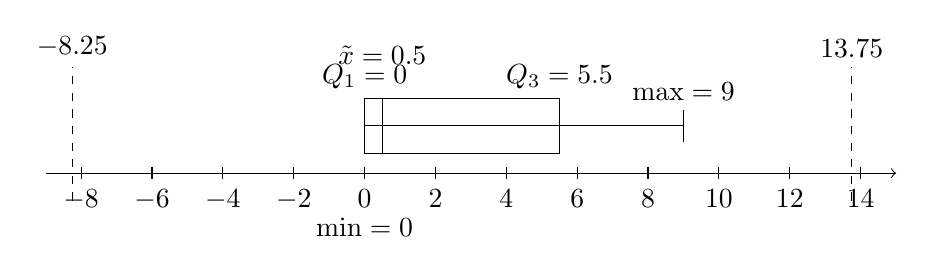
\begin{tikzpicture}[xscale=0.45,yscale=1]
\draw[->] (-9,0) -- (15,0);
\foreach \x in {-8,-6,-4,-2,0,2,4,6,8,10,12,14}
{
    \draw (\x,0.08) -- (\x,-0.08);
    \node[below] at (\x,-0.08) {\(\x\)};
}
\draw[dashed] (-8.25,-0.35) -- (-8.25,1.35);
\node[above] at (-8.25,1.35) {\(-8.25\)};
\draw[dashed] (13.75,-0.35) -- (13.75,1.35);
\node[above] at (13.75,1.35) {\(13.75\)};
\draw (0,0.6) -- (9,0.6);
\draw (0,0.25) rectangle (5.5,0.95);
\draw (0.5,0.25) -- (0.5,0.95);
\draw (0,0.4) -- (0,0.8);
\draw (9,0.4) -- (9,0.8);
\node[above] at (0,0.95) {\(Q_1=0\)};
\node[above] at (0.5,1.25) {\(\tilde{x}=0.5\)};
\node[above] at (5.5,0.95) {\(Q_3=5.5\)};
\node[above] at (9,0.8) {\(\max=9\)};
\node[below] at (0,-0.45) {\(\min=0\)};
\end{tikzpicture}
\end{center}

\newpage
\section*{Problem 21}

\textbf{Question.} To compare Glipizide and Jardiance with a placebo control group, 18 diabetics were randomly assigned into three groups of 6. The morning blood-sugar readings are shown below. Test at a $1\%$ significance level whether all three population mean blood-sugar levels are the same.
\[
\begin{array}{c|ccc}
& \text{Placebo} & \text{Glipizide} & \text{Jardiance}\\
\hline
1 & 137 & 128 & 119\\
2 & 161 & 139 & 112\\
3 & 155 & 121 & 123\\
4 & 179 & 146 & 108\\
5 & 144 & 151 & 128\\
6 & 150 & 125 & 132
\end{array}
\]

\textbf{Solution.} Test whether the three population mean blood-sugar levels are the same.
\[
H_0:\mu_1=\mu_2=\mu_3
\]
versus
\[
H_a:\text{at least one population mean is different}.
\]

The sample means are
\[
\bar x_1=\frac{137+161+155+179+144+150}{6}=154.3333,
\]
\[
\bar x_2=\frac{128+139+121+146+151+125}{6}=135,
\]
and
\[
\bar x_3=\frac{119+112+123+108+128+132}{6}=120.3333.
\]
The grand mean is
\[
\bar x_{\cdot\cdot}=\frac{926+810+722}{18}=136.5556.
\]

The treatment sum of squares is
\[
SSTr=\sum_{i=1}^{3}n_i(\bar x_i-\bar x_{\cdot\cdot})^2.
\]
Thus,
\[
SSTr=6(154.3333-136.5556)^2+6(135-136.5556)^2+6(120.3333-136.5556)^2.
\]
So,
\[
SSTr=3489.7778.
\]
The error sum of squares is
\[
SSE=\sum_{i=1}^{3}\sum_{j=1}^{6}(x_{ij}-\bar x_i)^2.
\]
Computing within each group,
\[
SSE=2242.6667.
\]

The degrees of freedom are
\[
df_{Tr}=k-1=3-1=2,
\]
and
\[
df_E=N-k=18-3=15.
\]
Therefore,
\[
MSTr=\frac{SSTr}{df_{Tr}}=\frac{3489.7778}{2}=1744.8889,
\]
and
\[
MSE=\frac{SSE}{df_E}=\frac{2242.6667}{15}=149.5111.
\]
The ANOVA test statistic is
\[
F=\frac{MSTr}{MSE}=\frac{1744.8889}{149.5111}=11.6706.
\]

The ANOVA table is
\[
\begin{array}{c|cccc}
\text{Source} & df & SS & MS & F\\
\hline
\text{Treatment} & 2 & 3489.7778 & 1744.8889 & 11.6706\\
\text{Error} & 15 & 2242.6667 & 149.5111 & \\
\text{Total} & 17 & 5732.4444 & &
\end{array}
\]

At the $1\%$ significance level,
\[
F_{0.01,2,15}=6.3589.
\]
The rejection rule is
\[
\text{reject }H_0\text{ if }F>6.3589.
\]
Since
\[
11.6706>6.3589,
\]
reject $H_0$. Therefore, at the $1\%$ significance level, there is sufficient evidence to conclude that not all three population mean blood-sugar levels are the same.
\[
\boxed{\text{Reject }H_0.}
\]

\end{document}
